% Author: Izaak Neutelings (June 2020)
% Inspiration:
%  https://courses.physics.ucsd.edu/2011/Summer/session1/physics2c/diffraction.pdf
%  https://tex.stackexchange.com/questions/201830/periodic-shading-in-tikz
\documentclass[border=3pt,tikz]{standalone}
% \usepackage[outline]{contour} % glow around text
\usepackage{physics}
\usepackage{xcolor}
\usepackage{etoolbox} %ifthen
\usetikzlibrary{calc}
\usetikzlibrary{arrows,arrows.meta}
\usetikzlibrary{decorations.markings}
% \usetikzlibrary{angles,quotes} % for pic (angle labels)
\usetikzlibrary{fadings}
\tikzset{>=latex} % for LaTeX arrow head
% \contourlength{1.4pt}

\colorlet{wall}{black}
\colorlet{myblue}{blue!70!black}
\colorlet{myorange}{orange!90!black!80}
\colorlet{myred}{red!70!black}
\colorlet{mydarkred}{red!50!black}
\colorlet{mylightgreen}{green!60!black!70}
\colorlet{mygreen}{green!60!black}
\colorlet{myredgrey}{red!50!black!80}
\colorlet{myshadow}{blue!30!black!90}
\tikzstyle{wave}=[myblue,thick]
\tikzstyle{mydashed}=[black!70,dashed,thin]
\tikzstyle{mymeas}=[{Latex[length=3,width=2]}-{Latex[length=3,width=2]},thin]
\tikzstyle{mysmallarr}=[-{Latex[length=3,width=2]}]

\newcommand\lineend[2]{
  \def\w{0.1} \def\c{30}
  \draw[mygreen] (#1)++(#2:\w) to[out=#2-180-\c,in=#2+\c] (#1)
                               to[out=#2+\c-180,in=#2-\c]++ (#2-180:\w);
}
\def\tick#1#2{\draw[thick] (#1) ++ (#2:0.1) --++ (#2-180:0.2)}



\begin{document}

% TWO SPLIT
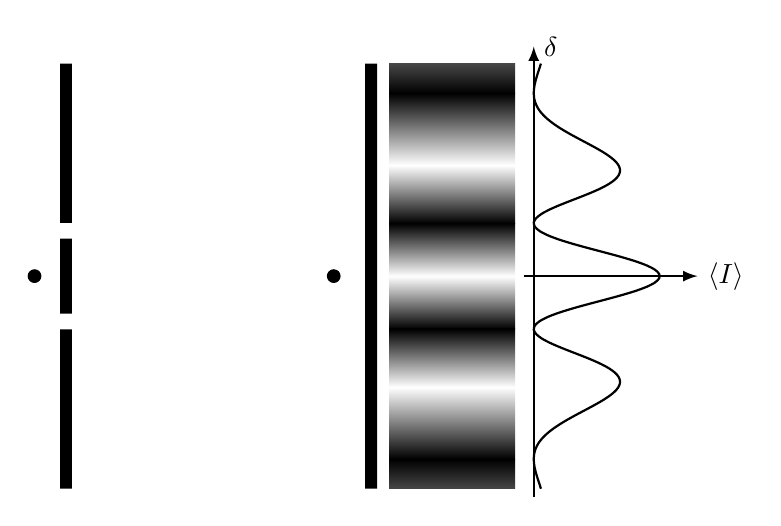
\begin{tikzpicture}[
    nodal/.style={black!75,dashed,very thin},
    declare function={
      xnode(\n,\dn,\lam,\f) = \lam/\f*sqrt( \n^2*(\f^2-\dn^2)+\n*\dn*(\f^2-\dn^2)+\dn^2*\f^2/2-(\f^4+\dn^4)/4 );
      ynode(\n,\dn,\lam,\a) = (2*\n*\dn+\dn^2)*\lam/(2*\f);
      intensity(\y,\lam,\a,\L) = exp(-\y*\y/5)*cos(180*\a*\y/(2*\lam*sqrt(\L*\L+\y*\y)))^2;
    }
  ]
  
  \def\L{3.8}       % distance between walls
  \def\H{5.4}       % total wall height
  \def\h{2.8}       % plane wave height
  \def\t{0.15}      % wall thickness
  \def\a{1.15}      % slit distance
  \def\d{0.20}      % slit size
  \def\N{21}        % number of waves
  \def\lambd{0.20}  % wavelength
  \def\R{\N*\lambd} % wave radius
  \def\Nlines{3}    % number of nodal lines
  \def\A{1.6}       % amplitude
  \def\nsamples{100}
  \def\ang{62}
  
    % PHOTONS
    \filldraw[fill=black] (-2*\lambd,0) circle (0.08);
    \filldraw[fill=black] (17*\lambd,0) circle (0.08);
  
  % WALL
  \fill[wall]
    (\t/2,\a/2-\d/2) rectangle (-\t/2,-\a/2+\d/2)
    (\t/2,\a/2+\d/2) rectangle (-\t/2,\H/2)
    (\t/2,-\a/2-\d/2) rectangle (-\t/2,-\H/2)
    (\L,-\H/2) rectangle (\L+\t,\H/2);
  
  % SHADE
  \begin{scope}[shift={(1.08*\L,0)}]
    \def\yz{\L/sqrt((\a/\lambd)^2-1)} % m = +- 1/2
    \def\yZ{\L/sqrt((\a/\lambd/2)^2-1)} % m = +- 1
    \clip (0,-\H/2) rectangle (1.1*\A,\H/2);
    \fill[white] (0,-\H/2) rectangle++ (\A,\H); % to fill seams
    \foreach \i [evaluate={\n=0.5*\i;\yn=\L/sqrt((\a/(2*\lambd*\n))^2-1);
                 }] in {1,...,\Nlines}{
      \ifodd\i % if even
        \fill[black] (0,{-\yn-0.1}) rectangle++ (\A,0.2); % to fill seams
        \fill[black] (0,{ \yn-0.1}) rectangle++ (\A,0.2); % to fill seams
      \fi
    }
    \path[left color=black,right color=black,middle color=white,shading angle={180}]
      (0,{-\yz}) rectangle (\A,{\yz});
    \foreach \i [evaluate={
                  \n=0.5*\i;
                  \m=0.5*(\i+1);
                  \yn=\L/sqrt((\a/(2*\lambd*\n))^2-1);
                  \ym=\L/sqrt((\a/(2*\lambd*\m))^2-1);
                  \dang=mod(\i,2)*180;
                 }] in {1,...,\Nlines}{
      \path[left color=black,right color=white,shading angle={\dang}]
        (0,\yn) rectangle (\A,\ym);
      \path[left color=black,right color=white,shading angle={180+\dang}]
        (0,-\yn) rectangle (\A,-\ym);
    }
  \end{scope}
  
  % INTENSITY
    \coordinate (NP0) at (\L,0);  % to avoid "Dimension too large error"
    \foreach \dn [evaluate={
                   \f=\a/\lambd;
                   \nmin=2.5+0.2*\dn; %0.501*(-\dn+\f)
                   \nmax=10; %(NP0)
                   \c=int(\dn<\f);
                   \y=\L/sqrt((\a/(\lambd*\dn))^2-1);
                 }] in {1,...,\Nlines}{
      \coordinate (NP+\dn) at (\L,\y);  % to avoid "Dimension too large error"
      \coordinate (NP-\dn) at (\L,-\y); % to avoid "Dimension too large error"
    }
    
  \begin{scope}[shift={(1.1*\L+1.1*\A,0)}]
    \draw[->,thick] (-0.08*\A,0) -- (1.3*\A,0) node[right=0] {$\langle I\rangle$}; % I axis
    \draw[->,thick] (0,-0.52*\H) -- (0,0.54*\H) node[right] {$\delta$}; % y axis
    \draw[thick,variable=\y,samples=\nsamples,smooth,domain=-\H/2:\H/2]
      plot({\A*intensity(\y,\lambd,\a,\L)},\y);
  \end{scope}

    \end{tikzpicture}


\end{document}